\section{Computação Gráfica e Modelagem 3D}
%%------------------------------------------------Introducao--------------------------------------------------------%%%%
	Computação gráfica é a representação e manipulação de dados utilizando um computador, com ajuda de \textit{software} e \textit{hardware} especializados. O seu desenvolvimento facilitou a iteração humano-computador, melhorando o entendimento e a interpretação de uma variedade de tipos de dados\cite{comp_grafica_h}.

	Os desenvolvimentos na área de computação gráfica têm causado impactos em vários tipos de mídia, assim revolucionando as industrias de: animação, cinema e jogos. Ela também tem afetado outros seguimentos da vida do ser humano, tais como os exemplos descritos na Tabela~\ref{tab:comp_teoria}. 

\begin{table}
\centering
\caption{Diferentes ramos da computação gráfica.}
\begin{tabular}{|l|l|}
	\hline
	Área & Aplicações \\ \hline
	Medicina &  Exames, diagnósticos, estudo, planejamento de procedimentos\\ \hline
	Arquitetura & Perspectivas, projetos de interiores e paisagismo\\ \hline
	Engenharia & Em todas as suas áreas (mecânica, civil, aeronáutica etc.)\\ \hline
	Meteorologia & Previsão do tempo, reconhecimento de poluição\\ \hline
	Segurança Pública & Definição de estratégias, treinamento, reconhecimento\\ \hline
	Astronomia & Tratamento de imagens, modelagem de superfícies\\ \hline
	Artes & Efeitos especiais, modelagens criativas, esculturas e pinturas\\
	\hline
\end{tabular}
\label{tab:comp_teoria}
\end{table}

	Um dos importantes conceitos da computação gráfica é o da modelagem 3D, que é o processo matemático para representação de objetos tridimensionais via software. Estes modelos podem ser feitos manualmente ou automaticamente; o processo manual tem semelhança com o método artístico de criação de esculturas, visto que o modelador constrói um objeto utilizando somente as ferramentais básicas disponíveis(tendo a criatividade como a ferramente principal). Já no processo automático o modelador utiliza-se de super \textit{scanners}, que capturam as característica de um objeto ou ambiente 3D deixando somente alguns ajustes por parte do modelador. 

%%%%%%%%%%%%%%%%%%%%%%%%%%%%%%%%%%%%%%%%%%%%%%%%%%%%%%%%%%%%%%%%%%%%%%%%%%%%%%%%%%%%%%%%%%%%%%%%%%%%%%%%%%%%%%%%%%%%%%%%%%%%%%%%%%%%%%%%%%%
%%------------------------------------------------------Fim-Introducao-----------------------------------------------------------------%%%%
%%%%%%%%%%%%%%%%%%%%%%%%%%%%%%%%%%%%%%%%%%%%%%%%%%%%%%%%%%%%%%%%%%%%%%%%%%%%%%%%%%%%%%%%%%%%%%%%%%%%%%%%%%%%%%%%%%%%%%%%%%%%%%%%%%%%%%%%%%%

\subsection{Transformações}
As transformações geométrica são ferramentas importantes em computação gráfica, pois permitem realizar ações do mundo real em um mundo virtual criado computacionalmente. Elas representam o mapeamento de um ou mais pontos de acordo com suas mudanças de posição~\cite{comp_grafica1}. As transformações mais usadas e conhecidas são: rotação, escala e translação. 

\subsubsection{Translação}
	A transformação geométrica mais básica é a de translação. É definida como a movimentação de todos os ponto, pertencente a um objeto, por uma mesma distância em uma mesma direção. Esta operação é dada pela equação ~(\ref{eq:translacao}), mostrando que quando certas quantidades ($T_x$, $T_y$ e $T_z$) são adicionadas às coordenadas ($x$, $y$ e $z$) (de todos os ponto de um dado objeto), obtêm-se uma nova posição transladada ($x'$, $y'$ e $z'$) para o ponto ($x$, $y$, $z$). A Figura~\ref{fg:trans} ilustra essa transformação. 

\begin{equation}\label{eq:translacao}
[x'\ y'\ z'] = [x\ y\ z] + [T_{x}\ T_{y}\ T_{z}]
\end{equation}

\begin{figure}[!ht]
	\centering
	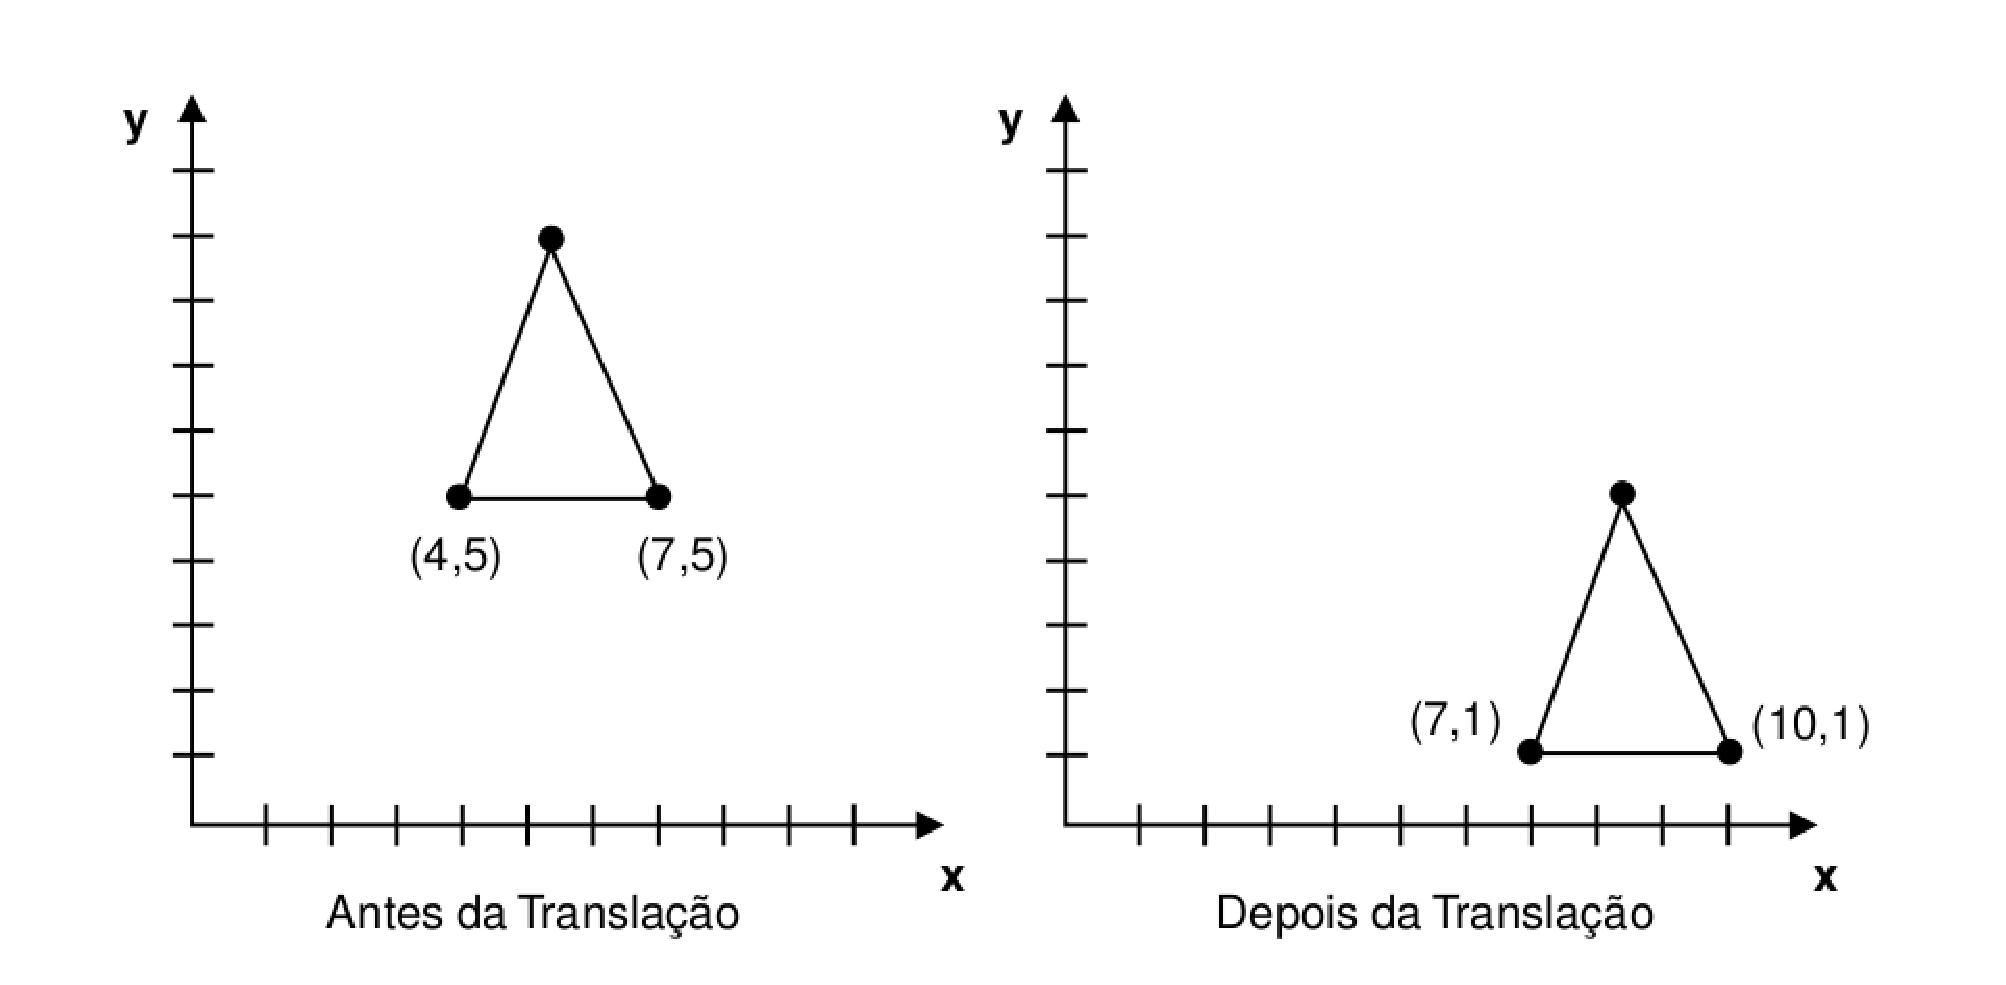
\includegraphics[scale=0.4]{trans}
	\caption{Operação de Translação 2D.}
	\label{fg:trans}
\end{figure} 

\subsubsection{Escala}
	A operação de escala está associada à mudança de dimensão (tamanho) dos objetos. Ela é representada pela equação matricial~(\ref{eq:escala}), a qual expressa que a multiplicação das dimensões atuais ($x$, $y$ e $z$) pelos fatores de escala ($S_x$, $S_y$ e $S_z$) tem como resultado um novo objeto escalado ($x'$, $y'$ e $z'$). A Figura~\ref{fg:escala} mostra o que ocorre quando um objeto é escalonado.

\begin{equation}\label{eq:escala}
	\begin{array}{c c c}
	[x' \ y' \ z'] = [x \ y \ z]
	\begin{bmatrix}
	S_x & 0 & 0   \\[0.2em]
	0 & S_y & 0   \\[0.2em]
	0 & 0 & S_z
	\end{bmatrix}
	\
	= [xS_x\ yS_y\ zS_z]
	\end{array}
\end{equation}

\begin{figure}[ht!]
	\centering
	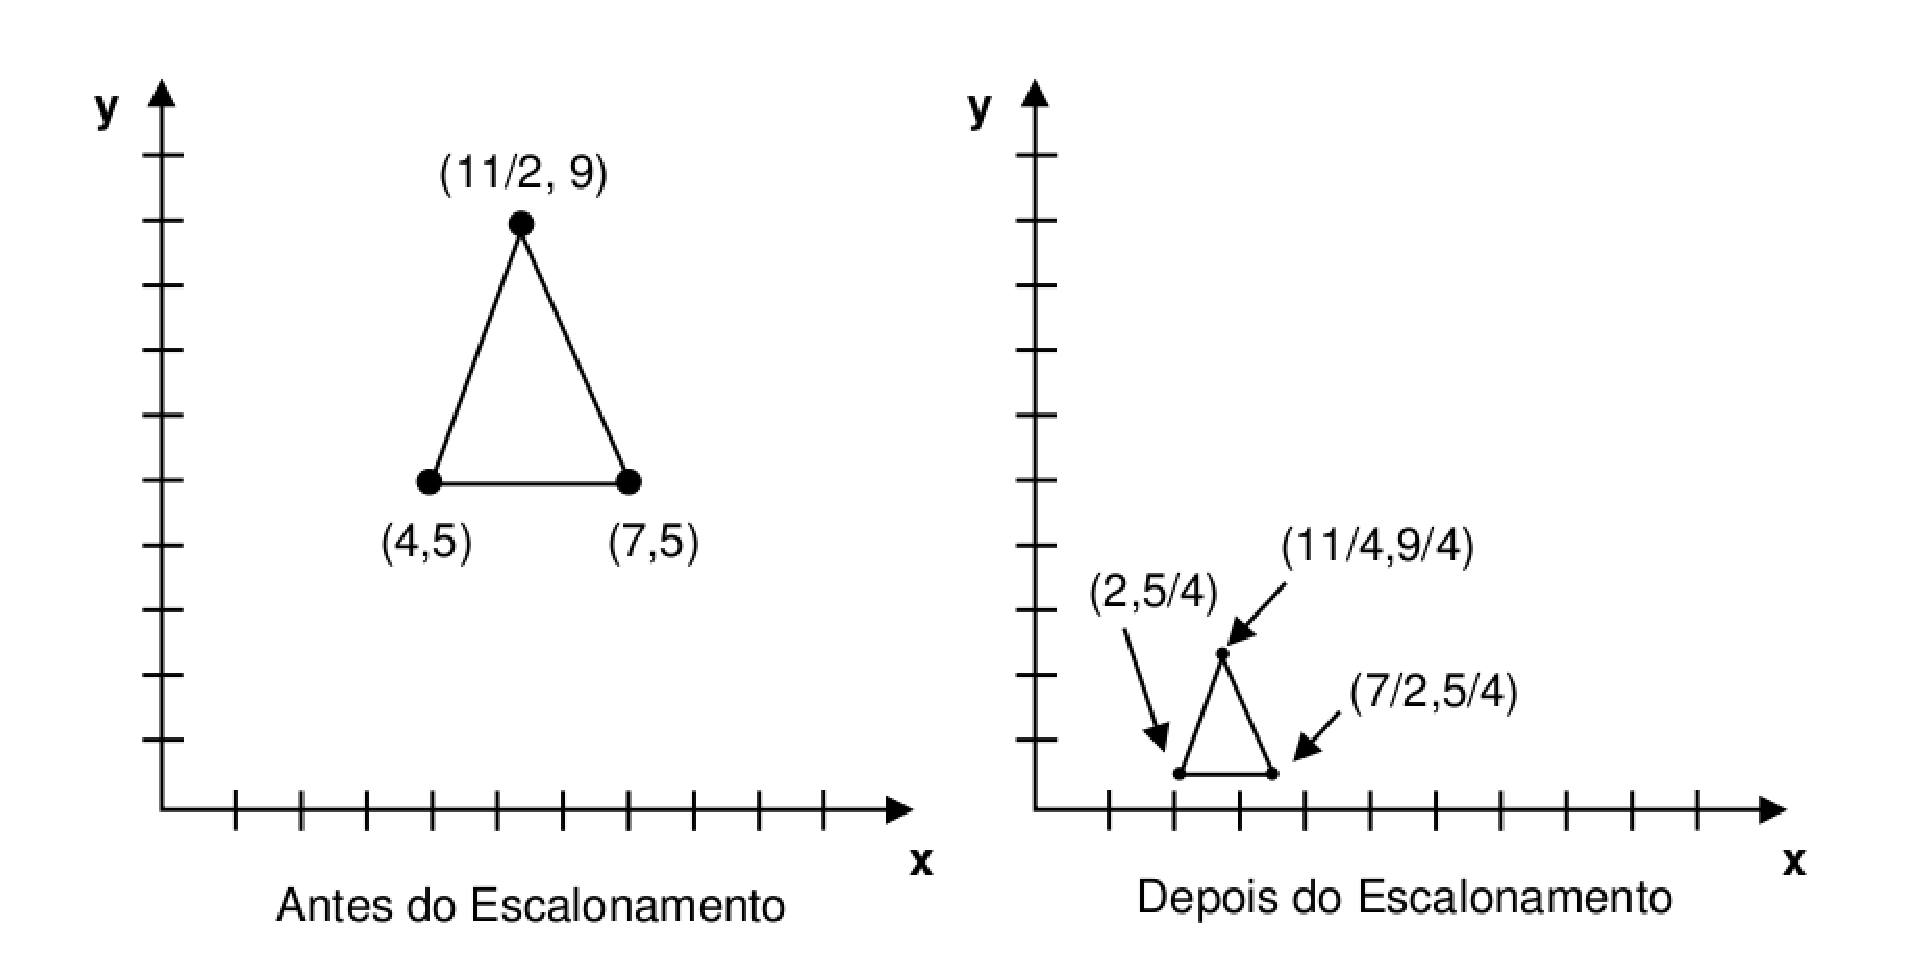
\includegraphics[scale=0.4]{escala}
	\caption{Operação de Escala 2D.}
	\label{fg:escala}
\end{figure} 

\subsubsection{Rotação}
	Rotação é a transformação que realiza o movimento giratório de um dado objeto entorno de um ponto fixo conhecido como centro de rotação. Esta transformação pode ser representada pelas formas matriciais~(\ref{eq:rotacao}), que mostram, respectivamente, as matrizes de rotação referentes aos eixos $x$, $y$ e $z$. A Figura~\ref{fg:rotacao} ilustra esta operação.

\begin{figure}[!ht]
	\centering
	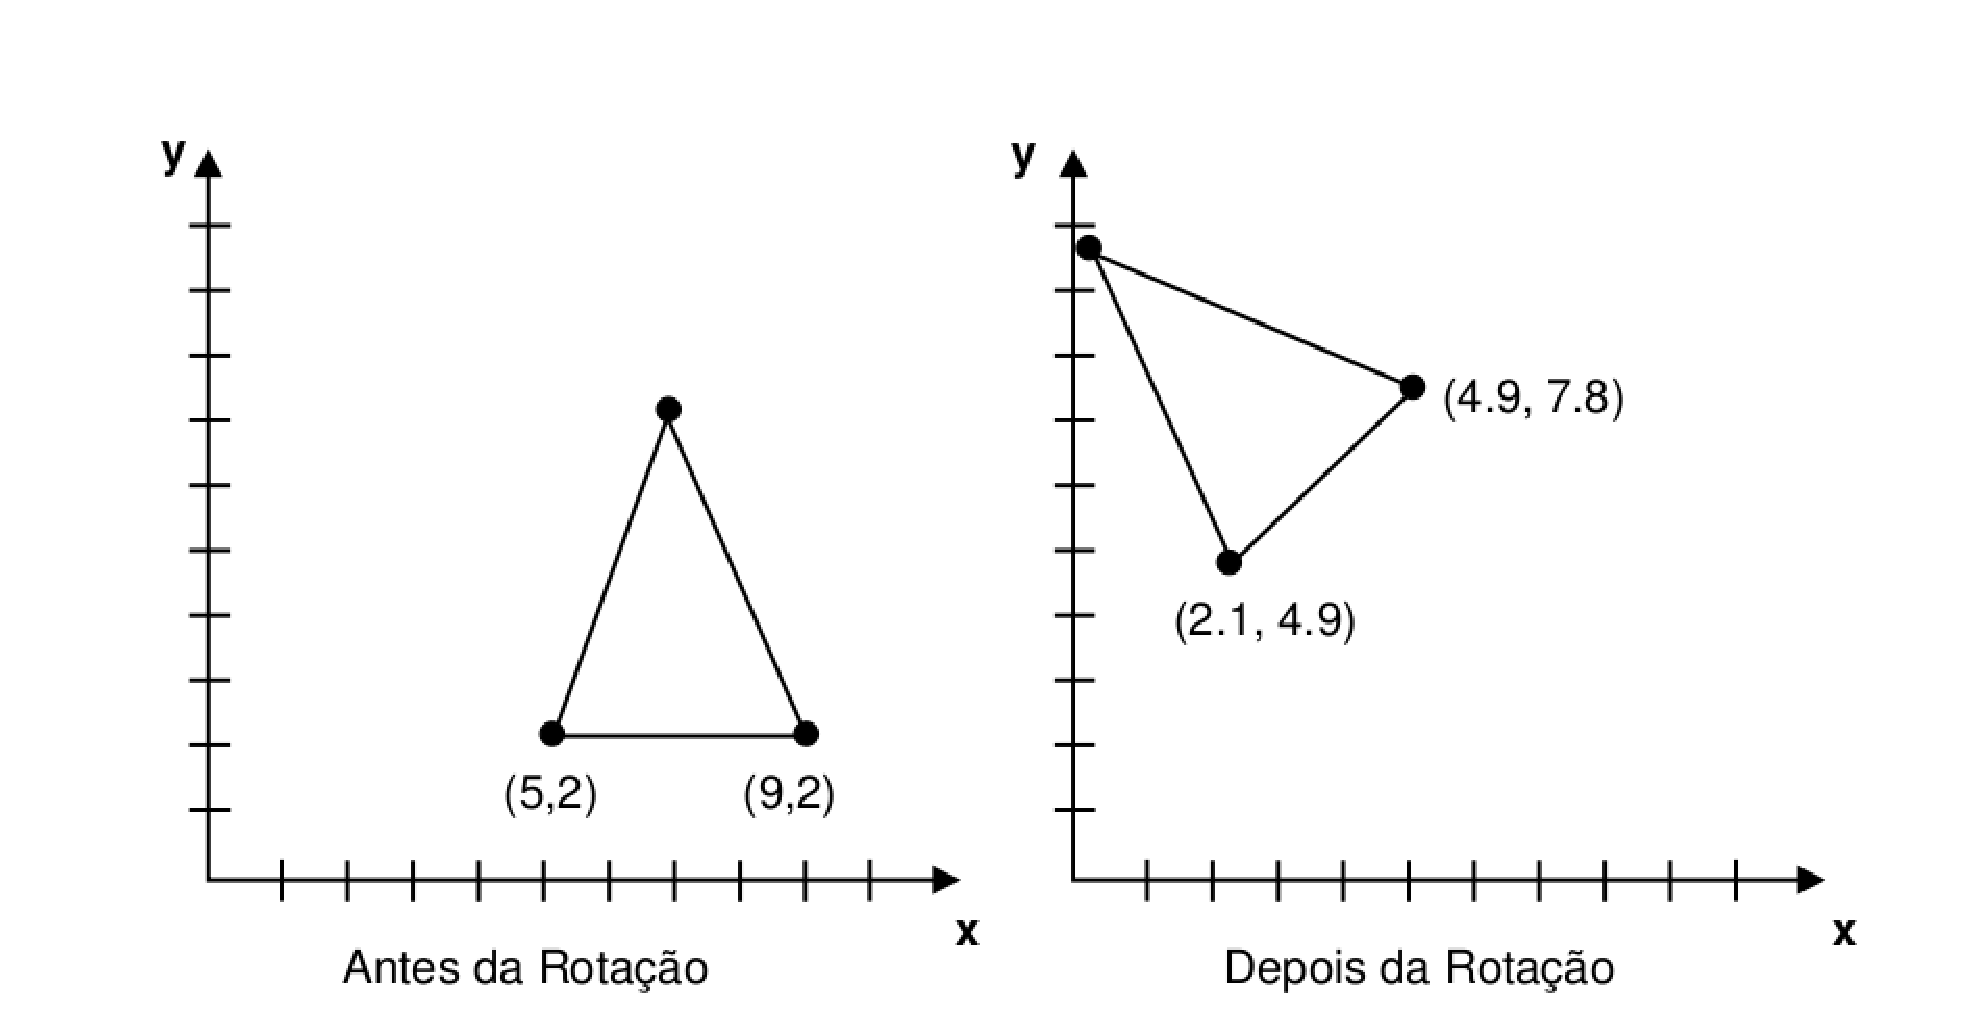
\includegraphics[scale=0.4]{rotacao}
	\caption{Operação de Rotação 2D.}
	\label{fg:rotacao}
\end{figure} 
\begin{center}
\begin{equation}\label{eq:rotacao}
	\begin{array}{c c c}
	R_x(\theta) = \begin{bmatrix}
	1 & 0 & 0   \\[0.2em]
	0 & \cos(\theta) & -\sin(\theta)    \\[0.2em]
	0 & \sin(\theta) & \cos(\theta) \\
	\end{bmatrix}
	, 
	R_y(\theta) = \begin{bmatrix}
	\cos(\theta) & 0 & \sin(\theta) \\[0.2em]
	0 & 1 & 0   \\[0.2em]
	-\sin(\theta) & 0 & \cos(\theta)\\
	\end{bmatrix}
	,
	R_z(\theta) = \begin{bmatrix}
	\cos(\theta) & -\sin(\theta) & 0\\[0.2em]
	\sin(\theta) & \cos(\theta) & 0\\[0.2em]
	0 & 0 & 1\\\ 
	\end{bmatrix}
	\end{array}
\end{equation}
\end{center}

%%%%%%%%%%%%%%%%%%%%%%%%%%%%%%%%%%%%%%%%%%%%%%%%%%%%%%%%%%%%%%%%%%%%%%%%%%%%%%%%%%%%%%%%%%%%%%%%%%%%%%%%%%%%%%%%%%%%%%%%%%%%%%%%%%%%%%%%%%%
%%------------------------------------------------------Fim-Transformacoes------------------------------------------------------------%%%%
%%%%%%%%%%%%%%%%%%%%%%%%%%%%%%%%%%%%%%%%%%%%%%%%%%%%%%%%%%%%%%%%%%%%%%%%%%%%%%%%%%%%%%%%%%%%%%%%%%%%%%%%%%%%%%%%%%%%%%%%%%%%%%%%%%%%%%%%%%%
\subsection{Representação de Sólidos}
	A representação de sólidos é um tópico de fundamental importância no aprendizado de modelagem 3D. Pois, dependendo da representação escolhida, pode-se tanto manipular quanto visualizar determinadas características de um objeto (sólido).

	A teoria de representação de sólidos é bastante ampla e possui um número muito grande de técnicas de representação. As técnicas utilizadas no desenvolvimento deste projeto são: Representação Aramada, Representação por Face, Representação por Polígono e Representação por Enumeração da Ocupação Espacial.

\subsubsection{Representação Armada ou \textit{Wireframe}}
	Nessa representação, visualiza-se somente as arestas e vértices que formam o objeto (Figura~\ref{fg:wireframe})~\cite{speck}. Sendo esta, a técnica mais simples de representação de objetos 3D.

	Suas vantagens e desvantagens estão associadas à visualização simplificada que esta proporcionada. Como vantagem, destaca-se a questão do custo computacional, visto que não há a necessidade de pintura das faces dos objetos (já que elas não existem neste modelo). A desvantagem é referente a ambiguidade na visualização dos objetos, como pode ser visto no exemplo apresentado na Figura~\ref{fg:wireframe2}. 

	Neste trabalho, a representação armada foi utilizada no evento de colisão, seção~\ref{sec:colisao}, para diferenciar a visualização de um objeto quando está selecionado.
\begin{figure}[ht!]
	\centering
	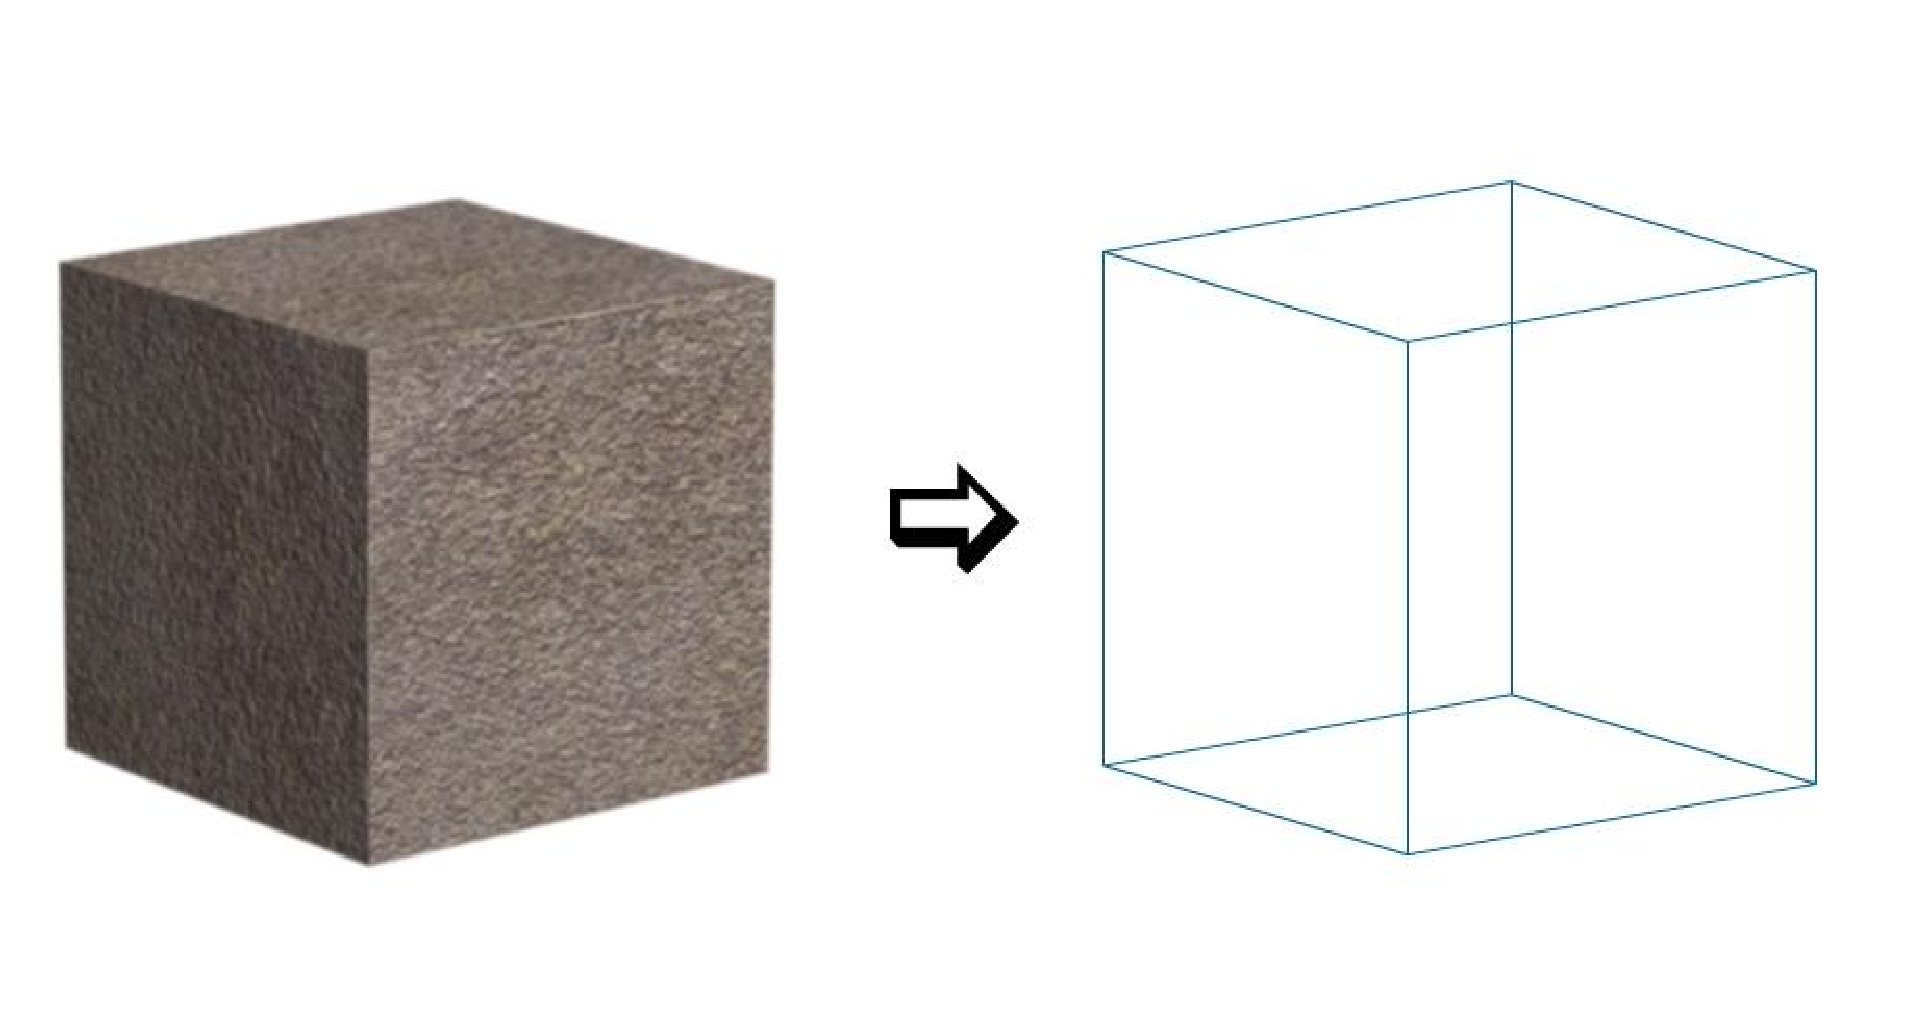
\includegraphics[scale=0.2]{wireframe}
	\caption{Representação Armada ou \textit{Wireframe}.}
	\label{fg:wireframe}
\end{figure} 
\begin{figure}[ht!]
	\centering
	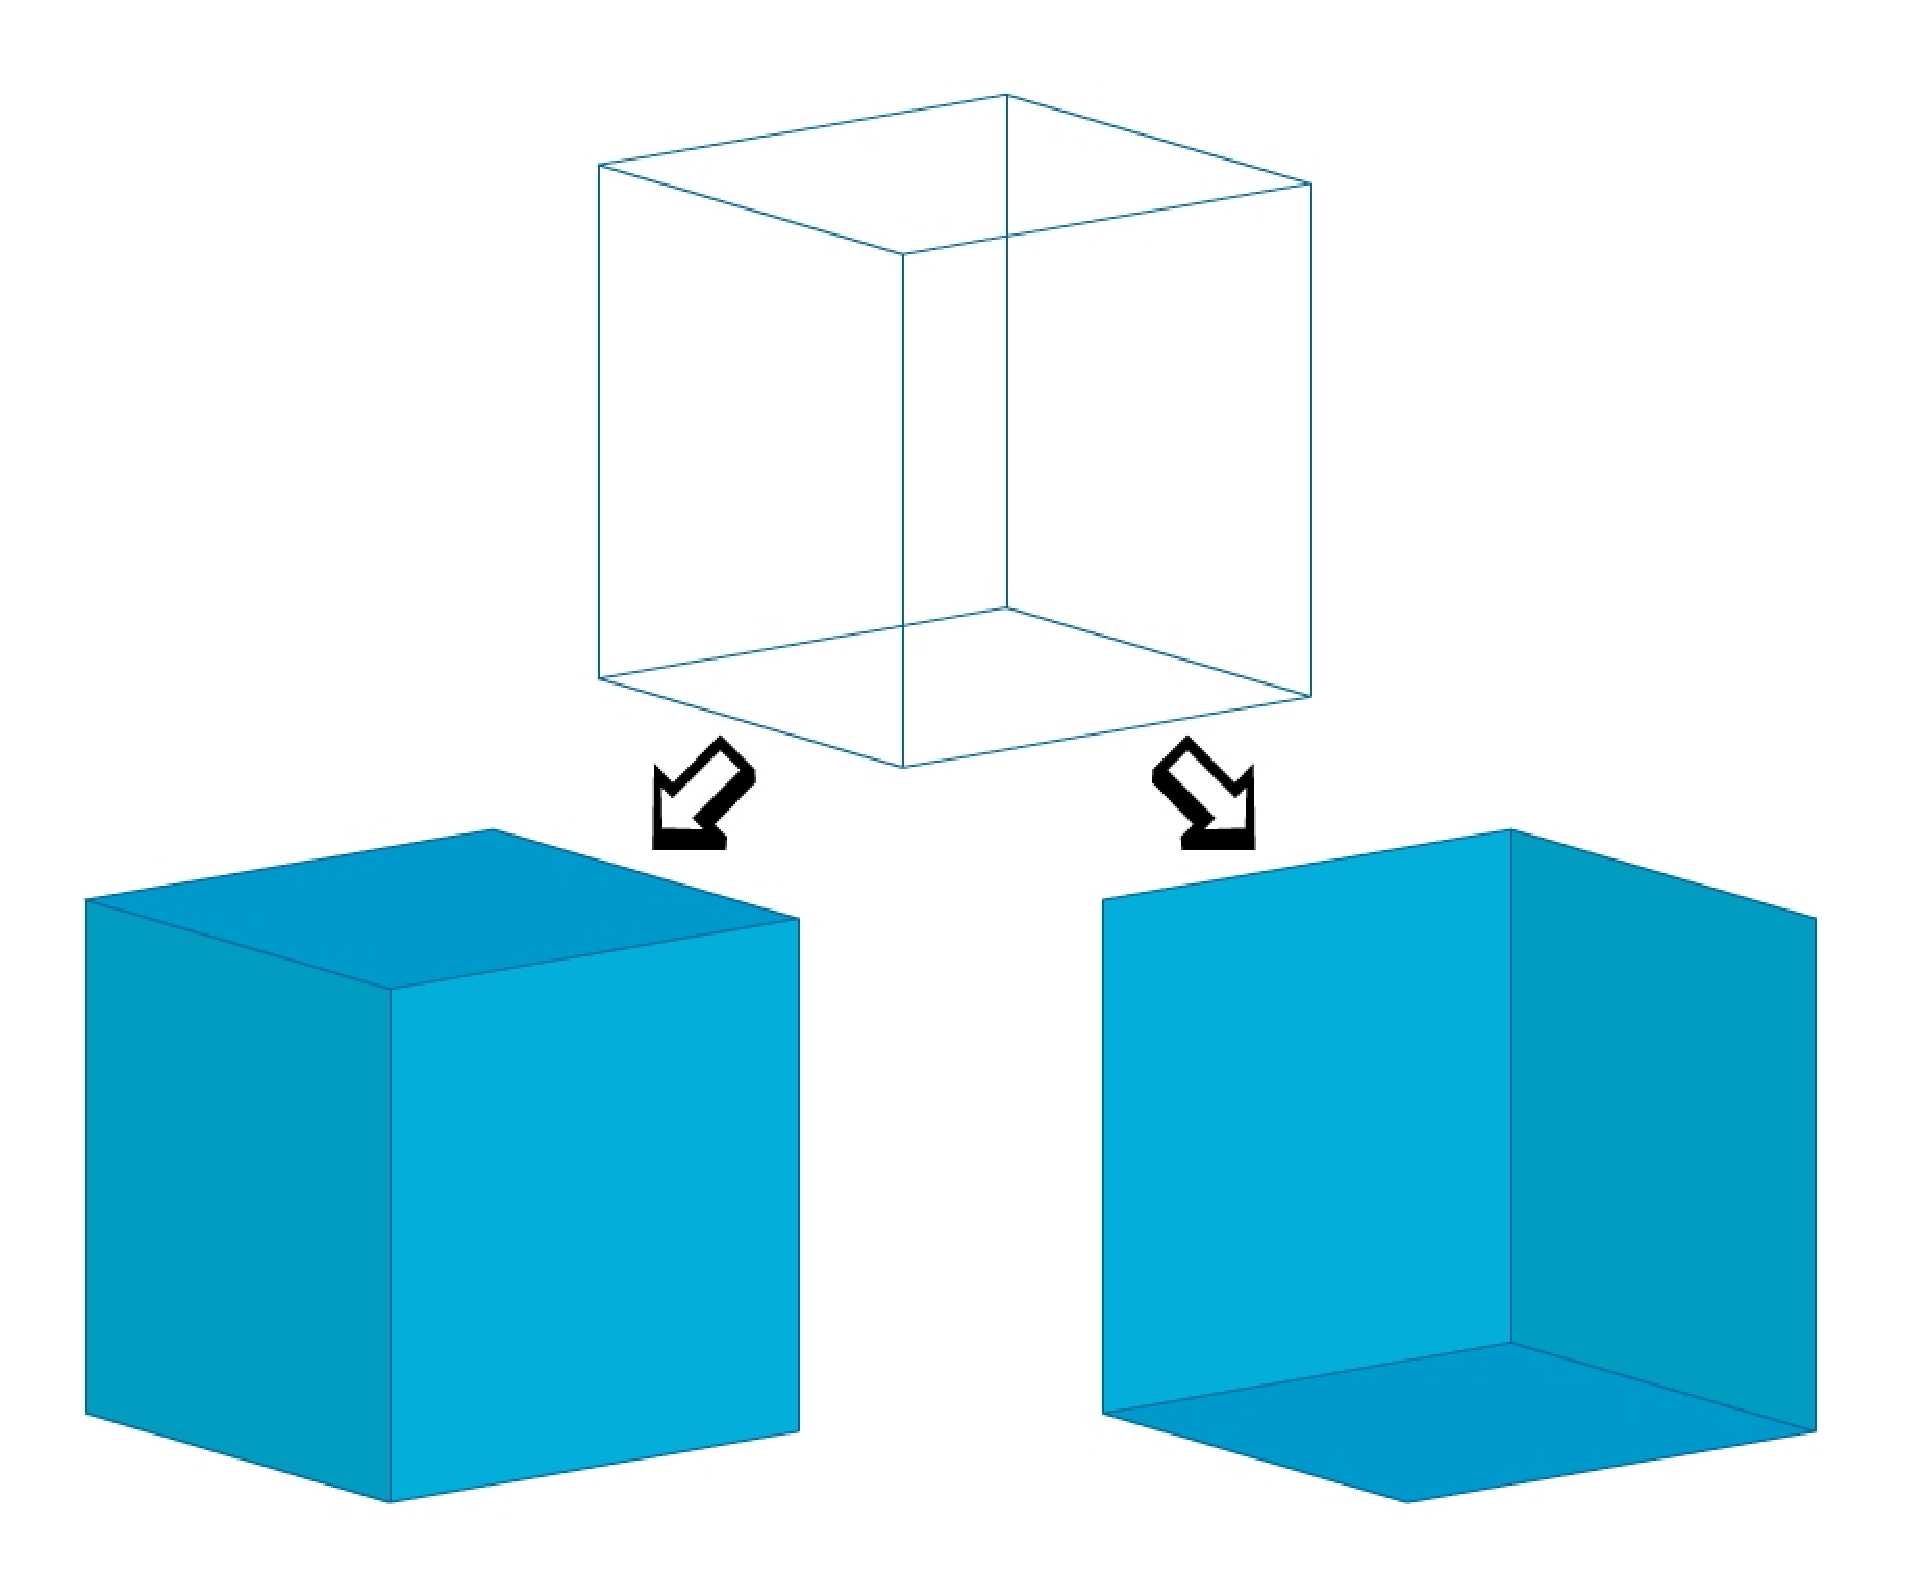
\includegraphics[scale=0.2]{wireframe2}
	\caption{Ambiguidade de representação de sólidos.}
	\label{fg:wireframe2}
\end{figure} 

\subsubsection{Representação por Faces} 
\label{sec:faces}
	Também conhecida com \textit{Boundary Representation} ou simplesmente \textit{B-rep}, essa técnica representa um modelo sólido por meio de suas fronteiras espaciais (Fig.~\ref{fg:faces}), tendo em geral uma superfície externa e uma convenção que define qual lado da superfície está o material sólido. Desta forma, um objeto sólido pode ser representado por faces, delimitadas por arestas, definidas por vértices~\cite{brep2}.
\begin{figure}[ht!]
	\centering
	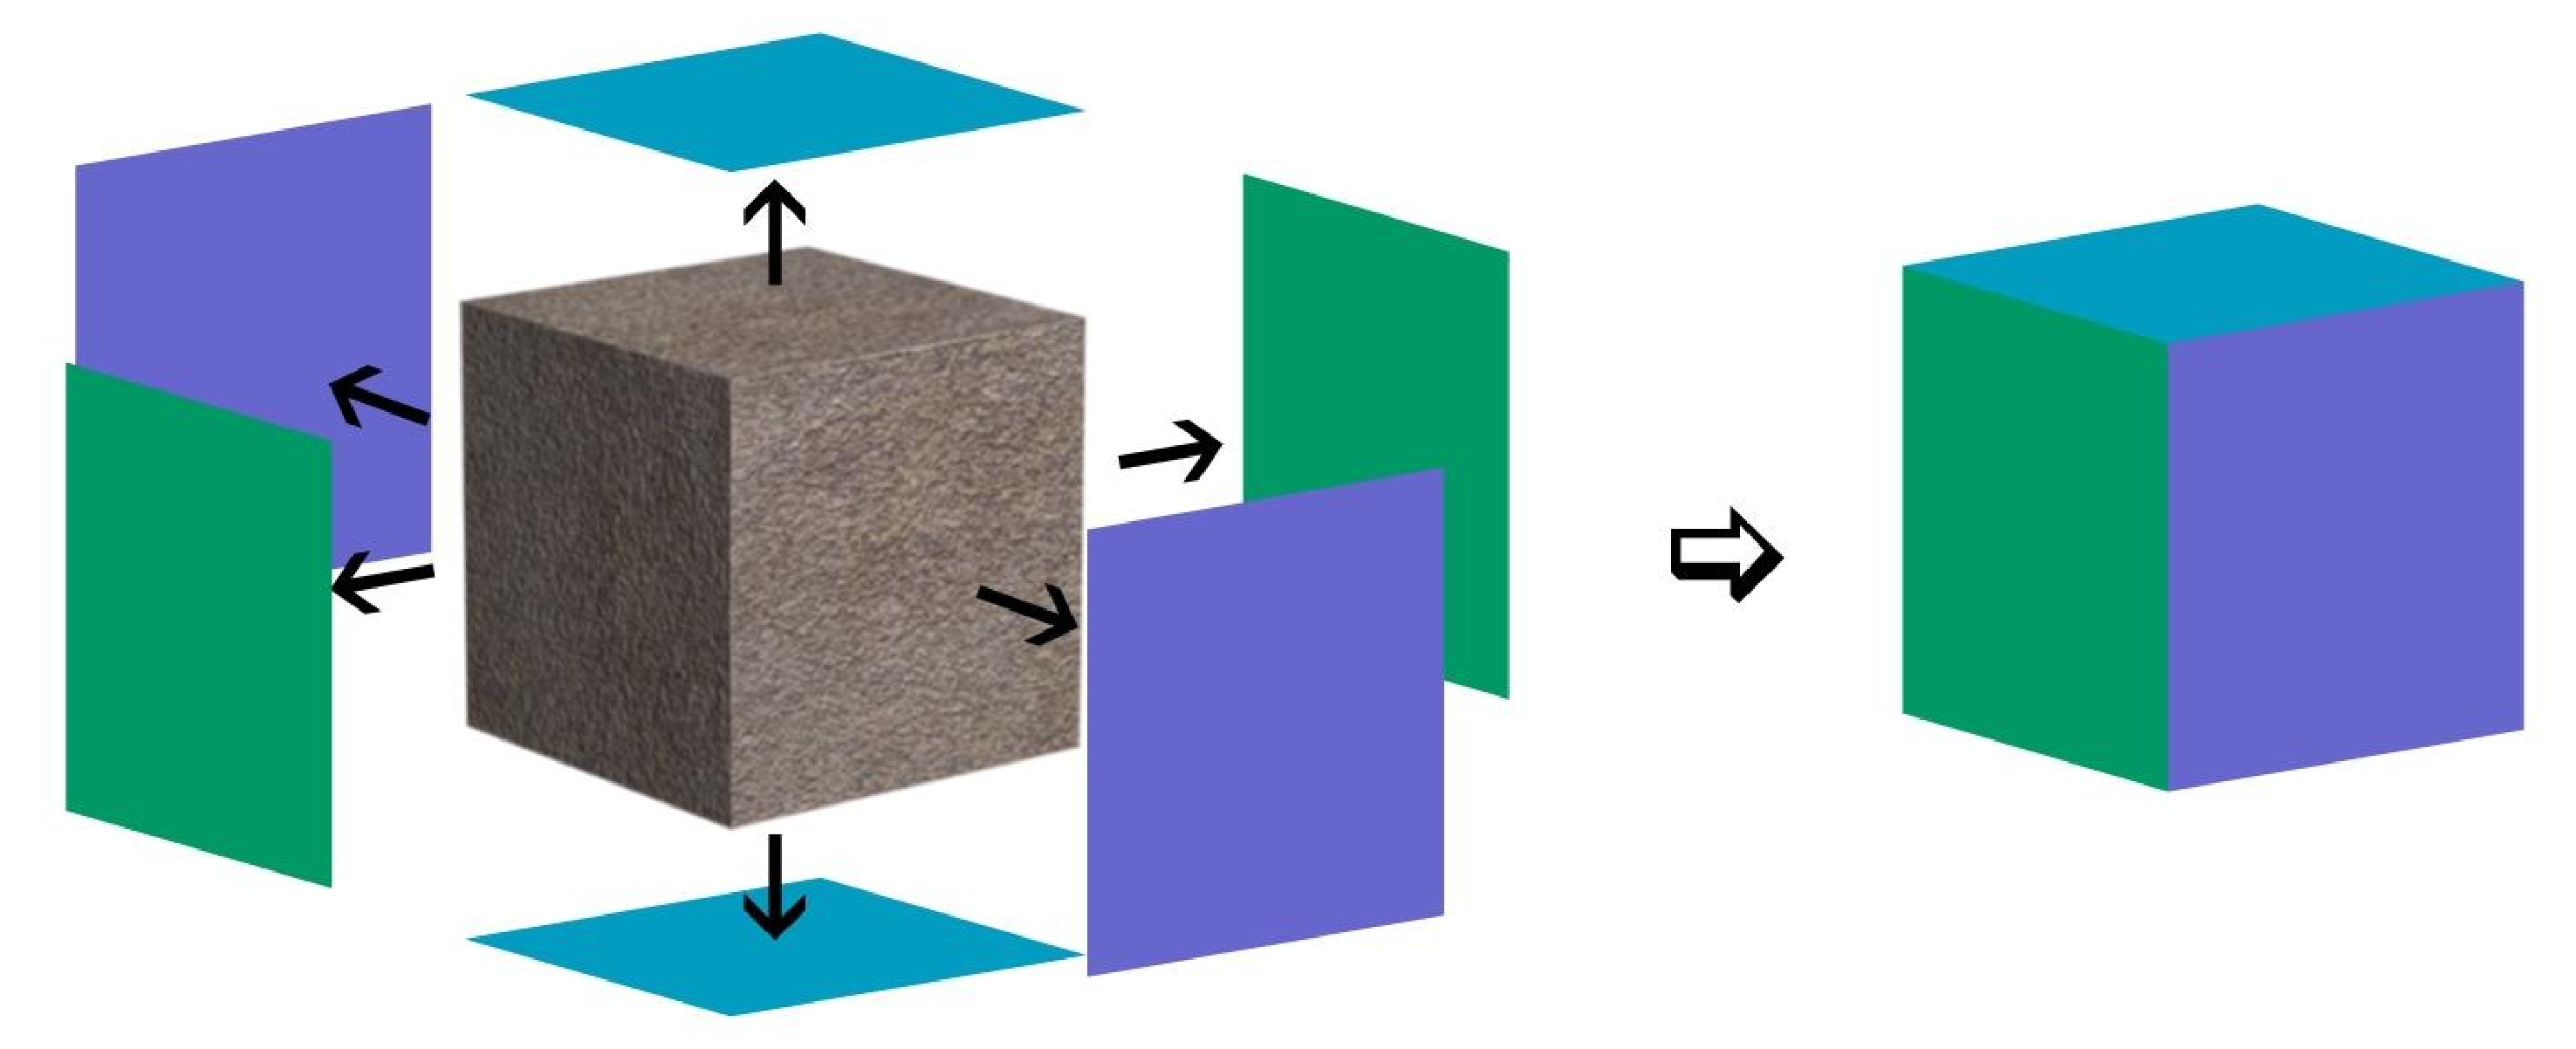
\includegraphics[scale=0.2]{faces}
	\caption{Representação por Faces.}
	\label{fg:faces}
\end{figure} 

	A primeira geração desta técnica, permitia representar sólidos somente por faces planas, o que limitava o número de formas geométricas que poderiam ser modeladas. Já a segunda geração, incluiu objetos primitivos com superfícies analíticas, possibilitando, assim, a criação de modelos um pouco mais complexos como cilindros, esferas, cones, etc.

	Foram realizados outros estudos, como intuito de que a técnica \textit{\textbf{B-Rep}} conseguisse modelar um maior número de formas geométricas, resultando em uma maior utilização deste método na modelagem de sólidos~\cite{brep2}. 

	Sua relevância nesse projeto, está associada ao entendimento da diferença entre o universo físico e o representativo (modelado), visto que, quando utiliza-se essa técnica, as informações referentes ao material sólido do objeto modelado não tem relevância.

\subsubsection{Representação Poligonal}
	Polígono vem do grego \textit{polys}, que significa muitos e \textit{gonos} que significa ângulos. Assim, esta representação é formada por figuras planas com muitos segmentos de reta e muitos ângulos. Então, pode-se construir sólidos com o polígono mais simples, o triângulo, ou mesmo com um mais complexo, com um número elevado de lados(Fig.~\ref{fg:poligonos}). Essa técnica pode ser considerada uma especificação do caso apresentado na seção~\ref{sec:faces}.
\begin{figure}[ht!]
	\centering
	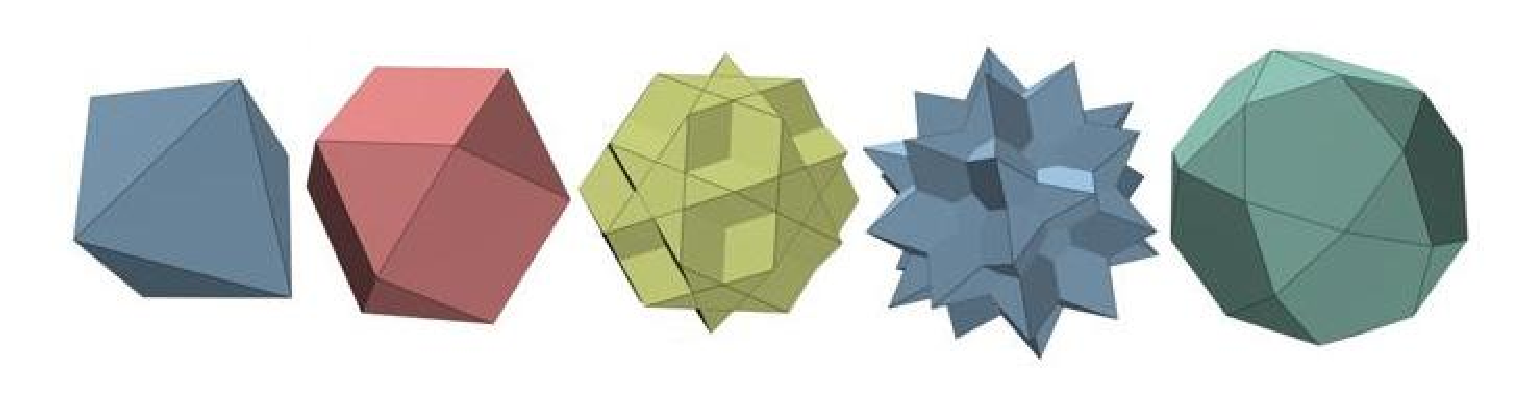
\includegraphics[scale=0.2]{poligonos}
	\caption{Representação Poligonal.}
	\label{fg:poligonos}
\end{figure} 

	\textit{Tessellation} é um das características dessa representação, significa preencher uma dada região através de várias repetições de um mesmo polígono, até não haver mais espaços em "branco". A maioria das máquinas de jogos utiliza a representação por faces triangulares. Isso se deve ao fato de esta necessitar de menos processamento e também por possibilitar a representação de grande parte dos tipos de contorno~\cite{traina}.

	A \textit{engine Irrlicht} se utiliza dessa técnica de representação para criar as malhas de seus objetos. A Figura~\ref{fg:tessellation}, ilustra o método de criação da malha cônica utilizando a técnica de representação poligonal.
\begin{figure}[ht!]
	\centering
	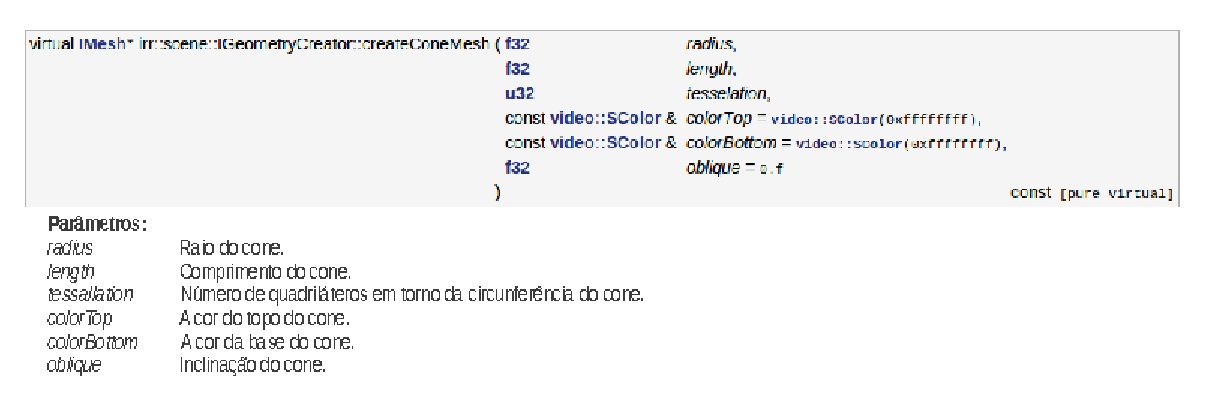
\includegraphics[scale=0.9]{tessellation}
	\caption{Método de criação da malha de um cone que usa a técnica de \textit{tessellation}~\cite{tesselation}.}
	\label{fg:tessellation}
\end{figure} 

\subsubsection{Representação por Enumeração da Ocupação Espacial}
	Esta técnica consiste na decomposição do espaço ocupado por um objeto em uma grade regular, formada por cubos(também chamados de \textit{voxels}) de dimensões iguais~\cite{ocupacaoespacial} , como está ilustrado pela imagem~\ref{fg:ocupacao_espacial}.
\begin{figure}[ht!]
	\centering
	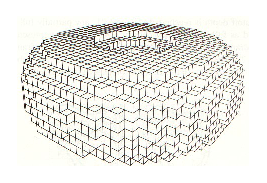
\includegraphics[scale=1]{ocupacao_espacial}
	\caption{Exemplo de objeto representado por enumeração da ocupação espacial}
	\label{fg:ocupacao_espacial}
\end{figure} 

	Quando um objeto é representado usando enumeração por ocupação espacial, controla-se somente a ausência ou presença da célula (cubo) em cada posição da grade. Desta forma, o objeto pode ser armazenado em uma lista de cubos que pertencem ao espaço por ele ocupado.

	Este modelo de representação permitiu a conexão do \textit{software} desenvolvido neste projeto com o simulador que utiliza o método FDTD (LANE-SAGS) . Esta união será melhor abordada na seção~\ref{sec:c_sags}.
%%%%%%%%%%%%%%%%%%%%%%%%%%%%%%%%%%%%%%%%%%%%%%%%%%%%%%%%%%%%%%%%%%%%%%%%%%%%%%%%%%%%%%%%%%%%%%%%%%%%%%%%%%%%%%%%%%%%%%%%%%%%%%%%%%%%%%%%%%%
%%-----------------------------------------------------fim-Representacao-solidos-------------------------------------------------------%%%%
%%%%%%%%%%%%%%%%%%%%%%%%%%%%%%%%%%%%%%%%%%%%%%%%%%%%%%%%%%%%%%%%%%%%%%%%%%%%%%%%%%%%%%%%%%%%%%%%%%%%%%%%%%%%%%%%%%%%%%%%%%%%%%%%%%%%%%%%%%%
\subsection{Realidade Virtual}
	O termo Realidade Virtual surgiu na década de 1980 pelo artista e cientista da computação Jaron Lanier, que uniu dois universos, que até então eram muito distantes: o mundo real e o virtual. Porém, há registros de trabalhos anteriores a essa denominação. Um deles é o primeiro capacete que permitia imersão. Outro que não pode ser esquecido é o SENSORAMA, que foi construído na década de 1960 e tinha a capacidade de reproduzir imagens coloridas 3D, som, além de pode simular cheiros, ventania e vibrações durante os filmes.

	Mas o que é Realidade Virtual? É uma interface avançada que permite ao usuário navegar, modificar, interagir em tempo real com uma determinada aplicação que contenha objetos virtuais~\cite{rv}. Existem basicamente dois tipos de realidade virtual quanto o fator imersão: a imersiva e a não imersiva. A primeira é caracterizada por permitir ao usuário se sentir dentro do ambiente(através do uso de capacetes especiais, óculos, luvas, roupas, caves~\cite{cave}, sensores, dentre outros dispositivos). Já na segunda, isso não ocorre, utiliza-se mouse, teclado, monitores, etc \cite{aect}.

\subsubsection{Grafo de Cena}
	O grafo de cena é um conceito muito usado em computação gráfica, realidade virtual e teoria de jogos. Trata-se de uma estrutura de dados hierárquica que serve para representar as características e relações dos objetos que compõem um ambiente virtual tridimensional nas aplicações de computação gráfica. 

	Um ambiente virtual é uma representação de diversos aspectos do mundo abstrato ou virtual. Dentre estes aspectos estão a descrição geométrica, câmera, transformação, aparência, comportamento e iluminação, que são os mais relevantes em uma aplicação gráfica~\cite{ferreira}. Sendo assim, a representação de um cenário virtual é dada pela inserção de todos estes aspectos dentro do grafo de cena. Esta estrutura é formada por nós que compõem arestas, criado um conjunto em forma de árvore (grafo acíclico direcionado), Figura~\ref{fg:grafocena}.
\begin{figure}[ht!]
	\centering
	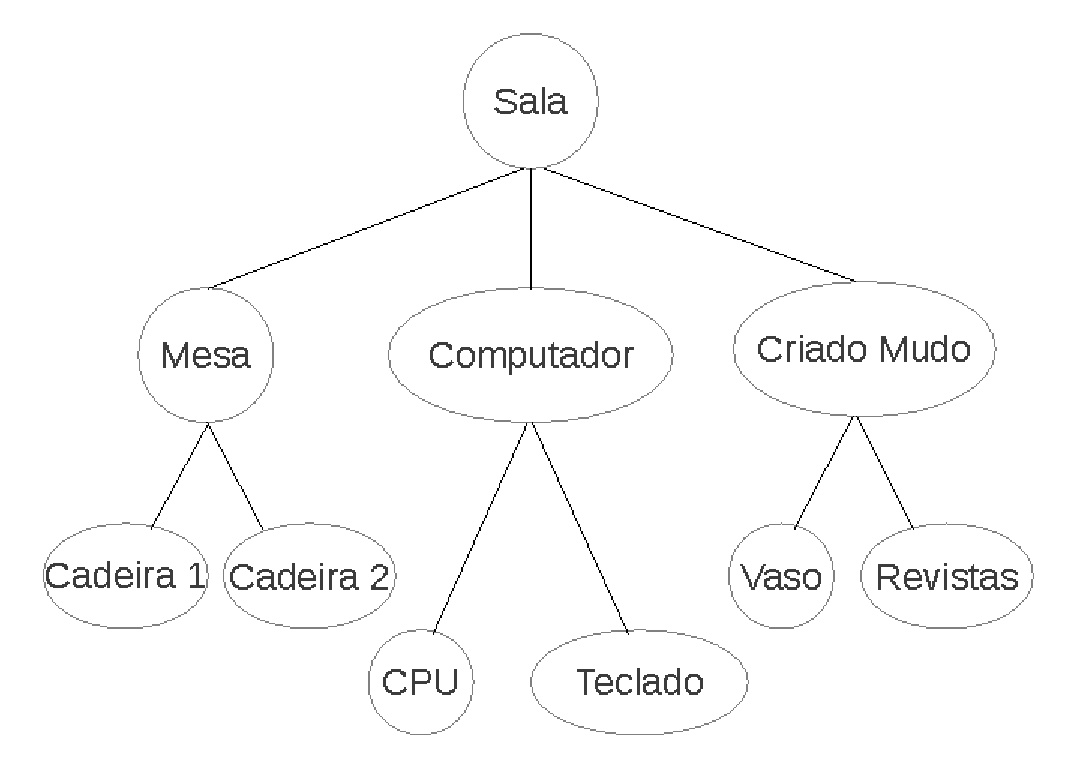
\includegraphics[scale=0.8]{grafocena}
	\caption{Grafo de cena de uma sala.}
	\label{fg:grafocena}
\end{figure} 
	Em um grafo de cena cada nó tem atributos que podem, ou não, influenciar seus nós conectados (nós filhos). Existe uma hierarquia na organização dos nós, que corresponde de forma semântica e espacial com o universo modelado.

	Com base nas características hierárquicas principais, os nós podem ser classificados em três categorias: nó raiz(é o primeiro nó, no qual todos os outros estão ligados de forma direta ou não), nó interno (geralmente contém informações de transformações 3D - rotação, escala e translação) e, por fim, há o nó folha (que por padrão contém as dados de representação geométrica dos objetos da cena).

	A propriedade fundamental dessa ferramenta é o que se chama de herança de estado. Ela determina que cada nó deve herdar as propriedades de todos os seus ancestrais provenientes do nó raiz, ou seja, se a posição do objeto principal for alterada, todos os objetos vinculados a ele irão modificar-se da mesma forma, mantendo suas posições relativas ao principal. Visualiza-se, então, que esta propriedade é bastante útil na organização de cenas 3D.

	A maioria dos motores de jogos, incluindo o escolhido para este projeto, utilizam as teorias de realidade virtual e grafo de cena. A justificativa está nas vantagens proporcionadas pelo uso desses conceitos. As principais vantagens podem ser vistas na Tabela\ref{tb:grafo_cena}.

\begin{table}
\centering
\caption{Vantagens proporcionadas pelo uso do grafo de cena.}
\begin{tabular}{|p{3cm}|p{8cm}|}
	\hline
	\multicolumn{2}{|c|}{\textbf{Vantagens}} \\ \hline
	\textbf{Produtividade} &  Gerencia e reduz o número de linhas de código que seriam necessárias para implementar
a mesma funcionalidade utilizando uma interface de baixo nível, como a OpenGL.\\ \hline
	\textbf{Portabilidade} &  Encapsula todas as tarefas de baixo nível, reduzindo e até 
excluindo a parte de código que é específica de uma plataforma.\\ \hline
	\textbf{Escalabilidade} &  Possibilita trabalhar tanto em máquinas com configurações básicas até supercomputadores\\ \hline
\end{tabular}
\label{tb:grafo_cena}
\end{table}

\section{Motor Gráfico}
	Um motor de jogos, dentro do conceito de engenharia de \textit{software}, é a parte do projeto que executa certas funcionalidades para um programa~(\textit{software}). No desenvolvimento de jogos, o motor se encarregará de interagir com o hardware gráfico, afim de dar o suporte necessário para visualização dos modelos, cuidará da entrada de dados do jogador, tratará todos os processos matemáticos envolvidos e gerenciar outros aspectos relacionados ao desenvolvimento de baixo nível, facilitando o desenvolvimento de um jogo ou sistema gráfico~\cite{engine}.

	Existem inúmeras definições para uma \textit{game engine}, porém todas elas convergem para as seguintes características principais:
\begin{itemize}
	\item Possibilitar o reaproveitamento de código.
	\item Promover uma fácil integração entre código e modelagem 3D.
	\item Permitir o desenvolvimento de  vários jogos, usando o mesmo motor. Todavia, é natural encontrar restrições em relação ao tipo de jogo que pode ser desenvolvido.
\end{itemize}

	A Tabela~\ref{tb:motor} mostra os principais motores gráficos utilizados atualmente.
\begin{table}
\centering
\caption{Principais motores de jogos.}
\begin{tabular}{|p{5cm}|p{9cm}|}
	\hline
	\textbf{Motores Tradicionais} & 3D GameStudio, BGE(Blender), C4 Engine, \textbf{Irrlicht}, NeoAxis Engine, Panda3D, Source, Torque Game Engine, Unreal Engine \\ \hline
	\textbf{Motores Proprietários} & 3D GameStudio, C4 Engine, DX Studio, EGO, Havok, NeoAxis Engine, Source, Unity, Truevision3D  \\ \hline
	\textbf{Motores de Código Aberto} & BGE (Blender), Crystal Space, \textbf{Irrlicht}, jME, ODE, OGRE, OpenSceneGraph, Panda3D, RPG Toolkit\\ 
	\hline
\end{tabular}
\label{tb:motor}
\end{table}

	A \textit{game engine} utilizada neste trabalho, foi o \textit{Irrlicht}. Esse motor de jogos foi escolhido, pelo conhecimento prévio obtido por meio do uso desta ferramenta em outros trabalhos e, principalmente, por ser \textit{open source} (código aberto).
%%%%%%%%%%%%%%%%%%%%%%%%%%%%%%%%%%%%%%%%%%%%%%%%%%%%%%%%%%%%%%%%%%%%%%%%%%%%%%%%%%%%%%%%%%%%%%%%%%%%%%%%%%%%%%%%%%%%%%%%%%%%%%%%%%%%%%%%%%%
%%------------------------------------------------------Fim-realidade-virtual----------------------------------------------------------%%%%
%%%%%%%%%%%%%%%%%%%%%%%%%%%%%%%%%%%%%%%%%%%%%%%%%%%%%%%%%%%%%%%%%%%%%%%%%%%%%%%%%%%%%%%%%%%%%%%%%%%%%%%%%%%%%%%%%%%%%%%%%%%%%%%%%%%%%%%%%%
\section{Método FDTD}
	Kane Yee criou o método FDTD (Finite-Differene Time-Domain Method), primeiramente chamado como Algorítimo de Yee, em 1966. Ésta técnica possibilita solucionar numericamente as equações de Maxwell de maneira simples e direta~\cite{rodrigo}. Tem como características principais: 
\begin{enumerate}
\item Distribuição geométrica discreta das componentes de campos Elétrico e Magnético em células, de maneira a satisfazer tanto a Lei de Faraday quanto a Lei de Ampère nas formas diferencial e integral.
\item Aproximação das derivadas espaciais e temporais por diferenças finitas, de forma a se obterem equações explicitas para a atualização temporal de todas as componentes de campo.
\end{enumerate}

	Porém, por algum tempo, esse método foi deixado de lado devido ao computacional muito alto. Aliado a isso, deve-se levar em consideração o contexto histórico em que ele se encontrava, onde os computadores ainda eram bem limitados. Mas, algum tempo depois, ressurgiu através dos trabalhos de dois cientistas, chamados Allen e Brodwin, que aplicaram essa técnica para problemas tridimensionais relacionados à interação eletromagnética com meios materiais\cite{allen}. Assim, novas técnicas apareceram e melhoram a abordagem do método, acompanhado da evolução dos computadores.

	Essa técnica tem sido usada desde então, em uma grande quantidade de aplicações. Entre elas estão: radares, antenas, fotônica, sistemas de telecomunicação, medicina, estruturas periódicas, sistemas de aterramento, entre várias outras\cite{taflove}.

	O método FDTD aplicado com intuito de simular propagação eletromagnética, utiliza as equações de Maxwell na forma diferencial,
\begin{equation}\label{eq:faraday}
	\overline{\nabla}\times\overline{E}=-\mu\frac{\partial \overline{H}}{\partial t},
\end{equation}
\begin{equation}\label{eq:ampere}
		\overline{\nabla}\times\overline{H}=\epsilon\frac{\partial \overline{E}}{\partial t} + \overline{J},
\end{equation}

\begin{flushleft}
Onde:
\end{flushleft}

	$\overline{J} = \sigma\overline{E}$, vetor densidade de corrente elétrica  de condução(ampere/m$^{2}$). As equações (\ref{eq:faraday}) e (\ref{eq:ampere}) expandidas em coordenadas retangulares, geram as equações escalares mostradas abaixo.

\begin{equation}\label{eq:hx}
	\frac{\partial H_x}{\partial t} = \frac{1}{\mu}(\frac{\partial E_y}{\partial z}-\frac{\partial E_z}{\partial y}),
\end{equation}
\begin{equation}
	\frac{\partial H_y}{\partial t} = \frac{1}{\mu}(\frac{\partial E_z}{\partial x}-\frac{\partial E_x}{\partial z}),
\end{equation}
\begin{equation}
	\frac{\partial H_z}{\partial t} = \frac{1}{\mu}(\frac{\partial E_x}{\partial y}-\frac{\partial E_y}{\partial x}),
\end{equation}

\begin{equation}
	\frac{\partial E_x}{\partial t} = \frac{1}{\epsilon}(\frac{\partial H_z}{\partial y}-\frac{\partial H_y}{\partial z} -\sigma E_x),
\end{equation}
\begin{equation}
	\frac{\partial E_y}{\partial t} = \frac{1}{\epsilon}(\frac{\partial H_x}{\partial z}-\frac{\partial H_z}{\partial x} -\sigma E_y),
\end{equation}
\begin{equation}\label{eq:ez}
	\frac{\partial E_z}{\partial t} = \frac{1}{\epsilon}(\frac{\partial H_y}{\partial x}-\frac{\partial H_x}{\partial y} -\sigma E_z)
\end{equation}

\begin{flushleft}
Onde:
\end{flushleft}

	$E_x, E_y, E_z$ e $H_x, H_y, H_z$ representam as componentes dos campos elétrico $\overline{E}$ e magnético $\overline{H}$, respectivamente. Essas componentes são funções do tempo $t$ e das três coordenadas cartesianas ($x,y,z$).

	A lei de Faraday, equação (\ref{eq:faraday}), informa que quando há variação no tempo do vetor $\overline{B}=\mu\overline{H}$ (vetor densidade de fluxo magnético, em teslas), surgem componentes de campo elétrico circulando em torno da(s) componente(s) deste vetor. Já a lei de Ampère, equação (\ref{eq:ampere}), informa que quando há variação no tempo do vetor $\overline{D}=\epsilon\overline{E}$ (vetor densidade de fluxo elétrico, em ) em certa direção e/ou a presença da fonte de corrente $\overline{J}$, esta causa circulação de campo magnético em torno da direção da(s) componente(s) deste vetor.

	Kane Yee se baseou nessa duas observações para definir seu esquema  de distribuição espacial  e temporal das componentes de campo de seu algoritmo. Sua representação geométrica, chamada de célula de Yee, está mostrada na Figura \ref{fg:celulaYee}\cite{rodrigo}.

\begin{figure}[ht!]
\centering
	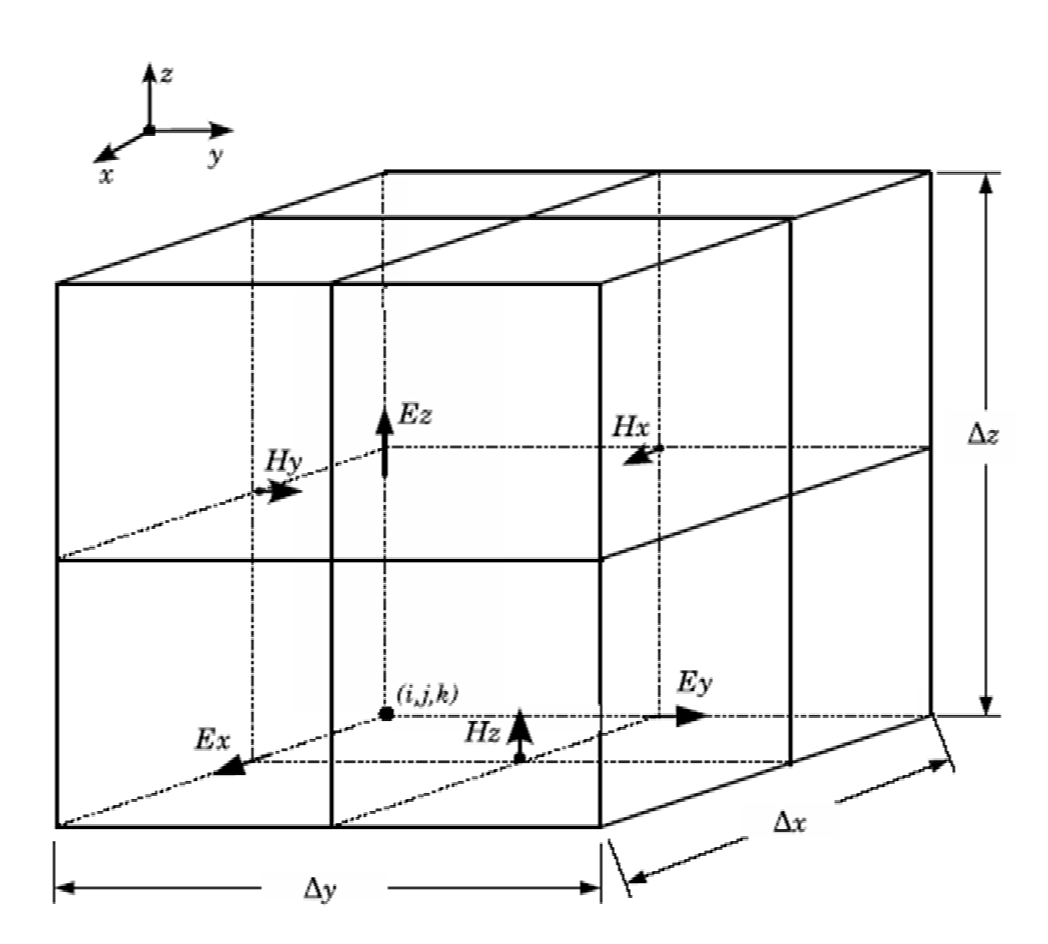
\includegraphics[scale=0.5]{celula}
	\caption{Célula Yee.}
	\label{fg:celulaYee}
\end{figure} 
		
	Para que possam ser realizadas simulações de propagação de onda através do método FDTD, é criada uma malha 3D formada por múltiplas células de Yee que preenchem toda região de análise. A Figura~\ref{fg:grade}\cite{almeida}, tem a finalidade de mostrar as componentes de campo de $\overline{E}$ e $\overline{H}$ distribuídas espacialmente na célula de Yee e a representação discreta de uma região do espaço através de múltiplas células.

\begin{figure}[ht!]
	\centering
	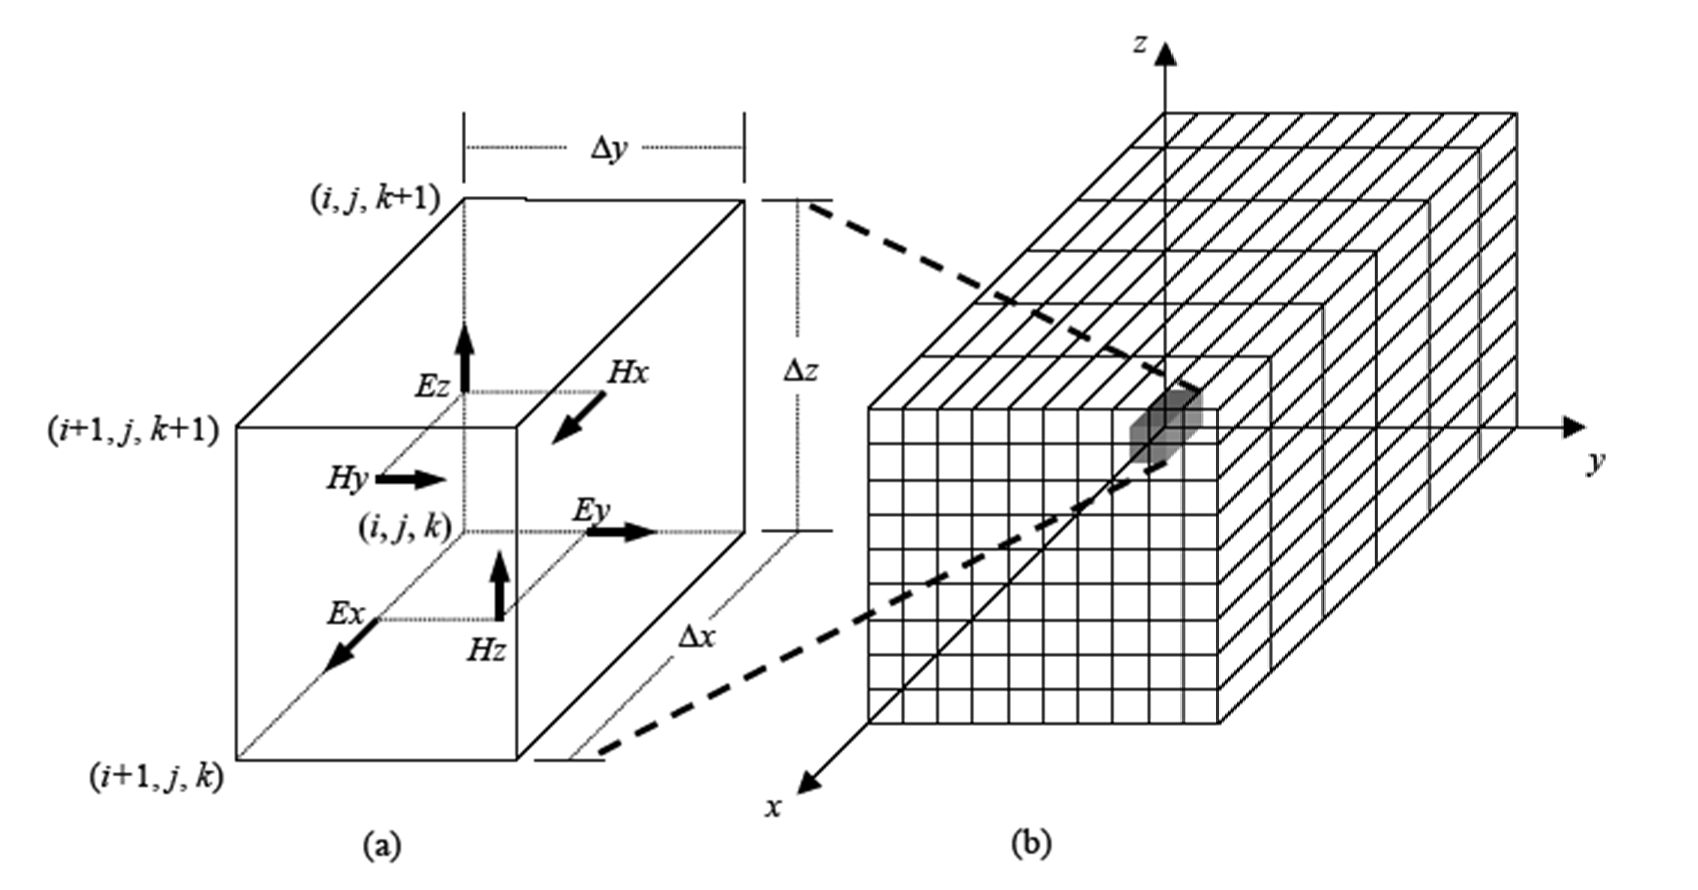
\includegraphics[scale=0.5]{Malha3D}
	\caption{(a) Posição das componentes dos campos elétrico e magnético em uma célula de Yee;(b) Célula no interior de uma malha 3-D.}
	\label{fg:grade}
\end{figure} 

	Como modo de referenciar uma célula nesta malha, utiliza-se os índices $i,j,k$ (discretos) para determinar a coordenada $x,y,z$ (em metros), através das relações $x = i.\Delta_x, y = j.\Delta_{y}$ e $z = k.\Delta_z$, onde  $\Delta_x,  \Delta_y$ e $\Delta_z$ são as dimensões das células de Yee(Figura\ref{fg:celulaYee})..

\subsection{Obtenção das Equações FDTD para $\overline{E}$ e $\overline{H}$}

	A análise das equações (\ref{eq:hx})-(\ref{eq:ez}) permite notar que suas derivadas podem ser aproximadas por derivadas centradas, tanto em relação ao tempo, quanto em relação ao espaço. A equação (\ref{eq:centrada}), é obtida a partir do trucamento de segunda ordem da série de Taylor, definindo o conceito de derivada centrada unidimensional.
\begin{equation}\label{eq:centrada}
	\frac{\partial f(x)}{\partial{x}} \approx \frac{f(x+\Delta_{x})-f(x-\Delta_{x})}{2\Delta_{x}}
\end{equation}

	Observando a equação (\ref{eq:centrada}) nota-se que a derivada no ponto $x$ em relação a $x$ pode ser aproximada por meio dos valores da função $f(x)$ nas coordenadas $x+\Delta_{x}$ e $x-\Delta_{x}$. Esta aproximação melhora com a diminuição do valor do $\Delta_{x}$. Então, uma função $F$ que dependa do tempo $t$ e das coordenadas espaciais ($x,y,z$) pode ser aproximada por uma função $F_a$ discreta, como representado matematicamente pela eq.(\ref{eq:func_f}).

\begin{equation}\label{eq:func_f}
	F(t,x,y,z) \approx F_{a}^{n}(i,j,k)
\end{equation}

	Utilizando a técnica de derivada centrada nas Equações (\ref{eq:hx})-(\ref{eq:ez}), obtêm-se as equações discretas para $\overline{H}$ e $\overline{E}$ :

\begin{equation}
	Hx_{(i,j+\frac{1}{2}, k+\frac{1}{2})}^{n+\frac{1}{2}} =
    Hx_{(i,j+\frac{1}{2}, k+\frac{1}{2})}^{n-\frac{1}{2}} +
    \frac{\Delta{t}}{\mu} \left [ \frac{Ey^{n}_{(i,j+\frac{1}{2}, k+1)} - Ey^{n}_{(i,j+\frac{1}{2}, k)}}{\Delta{z}}-
    \frac{Ez^{n}_{(i,j+1, k+\frac{1}{2})} - Ez^{n}_{(i,j, k+\frac{1}{2})}}{\Delta{y}} \right ]
\end{equation}\\
\begin{equation}
	Hy_{(i+\frac{1}{2},j, k+\frac{1}{2})}^{n+\frac{1}{2}} =
    Hy_{(i+\frac{1}{2}, j, k+\frac{1}{2})}^{n-\frac{1}{2}} +
    \frac{\Delta{t}}{\mu} \left [ \frac{Ez^{n}_{(i+1,j, k+\frac{1}{2})} - Ez^{n}_{(i,j, k+\frac{1}{2})}}{\Delta{x}}-
    \frac{Ex^{n}_{(i+\frac{1}{2},j, k+1)} - Ex^{n}_{(i+\frac{1}{2},j, k)}}{\Delta{z}} \right ]
\end{equation}\\
\begin{equation}
	Hx_{(i+\frac{1}{2},j+\frac{1}{2}, k)}^{n+\frac{1}{2}} =
    Hx_{(i+\frac{1}{2},j+\frac{1}{2}, k)}^{n-\frac{1}{2}} +
    \frac{\Delta{t}}{\mu} \left [ \frac{Ex^{n}_{(i+\frac{1}{2},j+1, k)} - Ex^{n}_{(i+\frac{1}{2},j, k)}}{\Delta{y}}-
    \frac{Ey^{n}_{(i+1,j+\frac{1}{2}, k)} - Ey^{n}_{(i,j+\frac{1}{2}, k)}}{\Delta{x}} \right ]
\end{equation}


\begin{equation}
\begin{array}{rcr}
	Ex_{(i+\frac{1}{2},j, k)}^{n+1} =
    Ex_{(i+\frac{1}{2},j, k)}^{n} +
    \frac{\Delta{t}}{\epsilon} \left [ \frac{Hz^{n+\frac{1}{2}}_{(i+\frac{1}{2},j+\frac{1}{2}, k)} - Hz^{n+\frac{1}{2}}_{(i+\frac{1}{2},j-\frac{1}{2}, k)}}{\Delta{y}}-
    \frac{Hy^{n+\frac{1}{2}}_{(i+\frac{1}{2},j, k+\frac{1}{2})} - Hy^{n+\frac{1}{2}}_{(i+\frac{1}{2},j, k-\frac{1}{2})}}{\Delta{z}} \right ]- \\
\sigma \Delta{t} 
\left [ \frac{Ex_{(i+\frac{1}{2}, j, k)}^{n+1} + Ex_{(i+\frac{1}{2}, j, k)}^{n}}{2} \right ]  
\end{array}
\end{equation}\\
\begin{equation}
\begin{array}{rcr}
	Ey_{(i,j+\frac{1}{2}, k)}^{n+1} =
    Ey_{(i,j+\frac{1}{2}, k)}^{n} +
    \frac{\Delta{t}}{\epsilon} \left [
	 \frac{Hx^{n+\frac{1}{2}}_{(i,j+\frac{1}{2}, k+\frac{1}{2})} - Hx^{n+\frac{1}{2}}_{(i,j+\frac{1}{2}, k-\frac{1}{2})}}{\Delta{z}}-
	 \frac{Hz^{n+\frac{1}{2}}_{(i+\frac{1}{2},j+\frac{1}{2}, k)} - Hz^{n+\frac{1}{2}}_{(i-\frac{1}{2},j+\frac{1}{2}, k)}}{\Delta{x}} 
\right ]-\\
\sigma \Delta{t} \left [ 
\frac{Ey_{(i, j+\frac{1}{2}, k)}^{n+1} + Ey_{(i, j+\frac{1}{2}, k)}^{n}}{2} 
\right ]
\end{array}  
\end{equation}\\
\begin{equation}
\begin{array}{rrr}
	Ez_{(i,j, k+\frac{1}{2})}^{n+1} =
    Ez_{(i,j, k+\frac{1}{2})}^{n} +
    \frac{\Delta{t}}{\epsilon} \left [ \frac{Hy^{n+\frac{1}{2}}_{(i,j+\frac{1}{2}, k+\frac{1}{2})} - Hy^{n+\frac{1}{2}}_{(i,j+\frac{1}{2}, k-\frac{1}{2})}}{\Delta{z}}-
    \frac{Hx^{n+\frac{1}{2}}_{(i+\frac{1}{2},j+\frac{1}{2}, k)} - Hx^{n+\frac{1}{2}}_{(i-\frac{1}{2},j+\frac{1}{2}, k)}}{\Delta{x}} \right ]-\\
\sigma \Delta{t} \left [ 
\frac{Ez_{(i, j, k+\frac{1}{2})}^{n+1} + Ez_{(i, j, k+\frac{1}{2})}^{n}}{2} 
\right ]
\end{array}
\end{equation}


%%%%%%%%%%%%%%%%%%%%%%%%%%%%%%%%%%%%%%%%%%%%%%%%%%%%%%%%%%%%%%%%%%%%%%%%%%%%%%%%%%%%%%%%%%%%%%%%%%%%%%%%%%%%%%%%%%%%%%%%%%%%%%%%%%%%%%%%%%%
%%------------------------------------------------------Fim-FDTD-----------------------------------------------------------------------%%%%
%%%%%%%%%%%%%%%%%%%%%%%%%%%%%%%%%%%%%%%%%%%%%%%%%%%%%%%%%%%%%%%%%%%%%%%%%%%%%%%%%%%%%%%%%%%%%%%%%%%%%%%%%%%%%%%%%%%%%%%%%%%%%%%%%%%%%%%%%%%
